\documentclass[oneside]{book}
\pagestyle{plain}

\usepackage{graphicx}
\usepackage[dutch]{babel}
\usepackage[nottoc]{tocbibind}
\usepackage{titlesec}
\usepackage[official]{eurosym}
\usepackage{graphicx}

%\newcommand{\itab}[1]{\hspace{0em}\rlap{#1}}
%\newcommand{\tab}[1]{\hspace{.25\textwidth}\rlap{#1}}
%\newcommand{\stab}[1]{\hspace{.05\textwidth}\rlap{#1}}
%\newcommand{\hl}{\begin{center} \line(1,0){350} \end{center}}
%\newcommand{\hl}{\hspace{\fill}\line(1,0){325}\hspace{\fill}}

\titleformat{\chapter}{\normalfont\Large\bfseries}{\chaptertitlename\ \thechapter{:\ }}{0pt}{\Large}{}
\titlespacing{\chapter}{0pt}{0pt}{1pt}

\title{Plan van aanpak\\
maze-runner\\
\normalsize voor de Hogeschool Rotterdam
}
\author{
	Stephan de Jonge (0901653@hr.nl)\\
	Stefan de Reuver (0890032@hr.nl)\\
	Victor Wernet (0903258@hr.nl)\\
	Nichelle Fleming (0902117@hr.nl)\\
	Wouter van der Plas (0898649@hr.nl)
}
\date{\today, Rotterdam}
%project naam toevoegen

\begin{document}
\maketitle
\tableofcontents


\chapter{Achtergrond}

%stakeholders Elvira(FIXME), van der Ven 
De Rotterdamse Hogeschool heeft ons de verbale en schriftelijke opdracht gegeven om een robot te bouwen die een doolhof kan doorkruisen.\\
Later werd hier aan toegevoegd dat de robot ook tot het randje van een afgrond moet kunnen rijden.\\
Dit moet gebeuren in de snelste tijd. Er is niet aangegeven of dit project deel is van een groter project.\\
het team, bestaande uit:\\
\begin{itemize}
	\item Wouter van der Plas (Teamleider)
	\item Nichelle Fleming (planner)
	\item Stephan de Jonge (programmeur)
	\item Victor Wernet (programmeur/bouwer)
	\item Stefan de Reuver (bouwer)
\end{itemize}	
Dit is de eerste keer dat deze groep in deze samenstelling werkt en samen een project van deze schaal doet.\\
\\
De naam komt van de film Maze Runner. Wij vonden dit passen om dat dit ook over een doolhof gaat.\\
\\
De stakeholders bestaan uit de projectgroep en de opdrachtgevers: mevrouw E. van der Ven en mevrouw L. Muilwijk.

\clearpage
\chapter{Projectresultaat}

Binnen dit project van 140 manuren willen wij één werkende Activitybot met twee configuraties één voor challenge A en één voor challenge B met bijbehorende project documentatie realiseren.

Dit project wordt uitgevoerd om ons(de studenten) praktische ervaring te laten opdoen binnen het vakgebied van de technische informatica.
Bovendien kan men maximaal vijf studiepunten behalen voor dit project.
Deze studiepunten hebben we nodig om onze opleiding te kunnen voltooien.

De doelstelling is om binnen de komende acht weken een werkende robot op te leveren met documentatie die rijdend een doolhof doorkruist met behulp van één of meerdere sensoren (Challenge A). 
Al het materiaal dat gebruikt wordt is verleend door de Hogeschool Rotterdam.\\
Ook is er een opdracht voor een tweede configuratie van dezelfde robot die zo dicht mogelijk tot een afgrond moet kunnen rijden zonder er van af te vallen (Challenge B).
\\
Na afronding van dit project, leveren wij een werkende robot af die een doolhof kan doorkruisen en een robot die tot een afgrond kan rijden.
\clearpage
\chapter{Projectactiviteiten}
{\large \textbf{ Plan voor het uitvoeren de opdracht opstellen:}}
\begin{itemize}
\item Initiele bespreking van de opdracht (2 uur)
\item Concept plan opstellen voor het uitvoeren van de opdracht (2 uur)
\item Bespreking wijzigingen (2 uur)
\item Plan bijstellen na het doorvoeren van de wijzigingen (2 uur)
\item Definitieve versie planning maken (2 uur)
\end{itemize}

{\large \textbf{Selecteren van de sensoren (onderzoeksopdracht):}}
\begin{itemize}
\item Testen van de infrarood, ultrasound en whiskers (5 uur)
\item Bepalen welke sensoren gebruikt zullen worden (1 uur)
\item Presentatie over de sensoren voorbereiden en geven (1 uur)
\end{itemize}

{\large \textbf{Opstellen van het plan van aanpak:}}
\begin{itemize}
\item Verzamelen en bestuderen van informatie (3 uur)
\item Gesprekken met de opdrachtgever en andere deskundigen (2 uur)
\item Concept plan van aanpak maken (3 uur)
\item Individueel feedback geven op het plan van aanpak van een andere projectgroep  (2 uur)
\item Bespreking van ontvangen feedbackformulieren (2 uur)
\item Definitieve versie plan van aanpak maken (4 uur)
\end{itemize}

{\large \textbf{Monteren van de sensoren:}}
\begin{itemize}
\item Plan montage opstellen (3 uur)
\item Montage 1ste concept (2 uur)
\item Montage bijstellen tot definitieve versie na testen (8 uur)
\end{itemize}

{\large \textbf{Programmeren van de code voor de montage:}}
\begin{itemize}
\item Plan sample code opstellen (2 uur)
\item Meerdere sample codes programmeren  voor montage 1ste concept (4 uur)
\item Code bijwerken tot definitieve versie na testen (8 uur)
\end{itemize}

\clearpage

{\large \textbf{Maken van het groepsdossier (rapporteren):}}
\begin{itemize}
\item Concept managementsamenvatting maken (3 uur)
\item Definitieve versie managementsamenvatting maken (4 uur)
\item Proefpresentatie voorbereiden en geven (4 uur)
\item Eindpresentatie voorbereiden en geven (3 uur)
\item Concept plan van aanpak, feedbackformulier ingevuld door medestudenten, feedbackformulier docent, definitief plan van aanpak en managementsamenvatting tot een groepsdossier samenstellen en inleveren (2 uur)
\end{itemize}

{\large \textbf{Maken van het individueel dossier:}}
\begin{itemize}
\item Een individueel procesverslag schrijven (3 uur)
\item Feedbackformulier proefpresentatie docent, samenvatting van de feedback van medestudenten, losse feedbackformulieren van medestudenten en \item individueel geschreven onderdeel managementsamenvatting samenstellen tot een individueel dossier en inleveren (2 uur)
\end{itemize}

{\large \textbf{Maken projectdossier (samenwerken):}}
\begin{itemize}
\item Individueel onderdeel managementsamenvatting schrijven (3 uur)
\item Reflectieverslag naar aanleiding van de thema’s “het geven van je mening”, “assertiviteit” en “het geven en ontvangen van feedback” schrijven (3 uur)
\item Verslagen samenstellen tot een projectdossier (1 uur)
\end{itemize}

\begin{table}[h]
\begin{tabular}{|l|l|l|l|l}
\cline{1-4}
code & Omschrijving & Uren & \begin{tabular}[c]{@{}l@{}}Kan\\ pas ná\end{tabular} &  \\ \cline{1-4}
A & \begin{tabular}[c]{@{}l@{}}Plan\\ voor het uitvoeren de opdracht opstellen\end{tabular} & 10 & - &  \\ \cline{1-4}
B & \begin{tabular}[c]{@{}l@{}}Selecteren\\ van de sensoren (onderzoeksopdracht)\end{tabular} & 7 & A &  \\ \cline{1-4}
C & Opstellen,van het plan van aanpak & 16 & A &  \\ \cline{1-4}
D & Monteren,van de sensoren & 13 & B &  \\ \cline{1-4}
E & \begin{tabular}[c]{@{}l@{}}Programmeren\\ van de code voor de montage\end{tabular} & 14 & D &  \\ \cline{1-4}
F & \begin{tabular}[c]{@{}l@{}}Maken\\ van het groepsdossier (rapporteren)\end{tabular} & 16 & \begin{tabular}[c]{@{}l@{}}A, B, C,\\ D en E\end{tabular} &  \\ \cline{1-4}
G & \begin{tabular}[c]{@{}l@{}}Maken\\ van het individueel dossier\end{tabular} & 5 & A,B, C, D en E &  \\ \cline{1-4}
H & \begin{tabular}[c]{@{}l@{}}Maken\\ projectdossier (samenwerken)\end{tabular} & 7 & A,B, C, D en E &  \\ \cline{1-4}
I & \begin{tabular}[c]{@{}l@{}}Challenge\\ uitvoeren\end{tabular} & 2 & \begin{tabular}[c]{@{}l@{}}A, B, C\\ en D\end{tabular} &  \\ \cline{1-4}
\end{tabular}
\end{table}

\clearpage
\chapter{Projectgrenzen}
Het project loopt van 20 november tot en met 24 januari. Hier zitten 2 weken vakantie tussen
waarin gewerkt kan worden, maar waarschijnlijk op een kleinere schaal dan de andere weken.\\
\\
Het maximale budget is vastgesteld op uren. Elke week wordt er maximaal 18 uur (per persoon) aan
gewerkt.
Dit cijfer is gebaseerd op het totaal aantal uren.
Dat zijn: 
\begin{itemize}
\item 32 uren voor de techniek binnen het schoolgebouw worden besteed
\item 25 uren verslaglegging, 4 uren voor de presentatie plus de voorbereiding
\item 64 totale uren voor zelf in te delen werkzaamheden(overal aan te besteden binnen het project)
\item 28 uren voor samenwerking en rapportage vaardigheden  
\item 1 uur voor de afsluiting en evaluatie
\end{itemize}
Alle materialen die voor het project worden gebruikt zijn verleend door de Hogeschool
Rotterdam.
We krijgen aan fysieke goederen: 1 Activitybot van Parallax, kabeltjes, sensoren, weerstanden, een
accu en een set mechano die vrij te gebruiken is.\\
\\
De concrete grenzen van het project zijn dat de robot zichzelf
autonoom door een doolhof heen kan navigeren met
de verschafte materialen. 
Bovendien moet er ook een tweede configuratie van de robot zijn die zo snel
mogelijk richting de rand van een tafel kan rijden en zichzelf op tijd stopt zodat hij er niet af valt.
Ook moet de documentatie zoals het plan van aanpak volledig aan de schriftelijke eisen voldoen, alle rapportage
en samenwerkingsopdrachten moeten
afgerond zijn en bovendien moet het geheel met een presentatie en een evaluatie zijn afgerond.
Als het laatst genoemde in orde en op tijd ingeleverd/gedaan is, dan is daarmee ook het project
succesvol afgerond.
Meer dan wat net is aangegeven als grens word niet gerealiseerd.

De randvoorwaarden voor het welslagen van dit project zijn: 
\begin{itemize}
\item We moeten van de Hogeschool op tijd alle materialen krijgen.
\item Er moet lang genoeg binnen de school gewerkt kunnen worden.
\item Alle faciliteiten die we binnen de school nodig hebben moeten beschikbaar zijn.
\item We moeten de juiste sturing van de project docent kunnen krijgen indien nodig.
\end{itemize}
\clearpage
\chapter{Tussenresultaten}
	de tussen resultaten die worden op geleverd zijn:
\begin{itemize}
	\item Concept Plan van Aanpak
	\item Definitief Plan van Aanpak
	\item Go/No-go op het Plan van Aanpak
	\item Onderzoeksresultaat sensoren
	\item Ontwerp sensoren Activity bot voor Challenge A
	\item Ontwerp sensoren Activity bot voor Challenge B
	\item Gerealiseerd ontwerp met alle benodigde sensoren aangesloten
	\item Concept code voor Challenge A en B
	\item Test resultaat(rapport) van concept code
	\item Complete versie van Concept code voor Challenge A en B
	\item Test resultaat(rapport) van volledige code
	\item Ontwerp eindpresentatie
	\item Volledige Activity bot mee laten doen aan Challenge A en B
	\item Complete eindpresentatie voordragen samen met de Activity bot
\end{itemize}
\clearpage
\chapter{Kwaliteit}
Om de kwaliteit van de tussenresultaten en eindresultaten te waarborgen wordt voor elk resultaat een rapport gemaakt dat vervolgens wordt gecontroleerd door de projectleider zodat er beslist kan worden of de kwaliteit van het resultaat aangepast moet worden.\\  

De resultaten worden ook besproken in een vergadering die het team wekelijks houd. In deze vergadering worden dan de behaalde resultaten besproken met het team en vervolgens een beslissing gemaakt om de kwaliteit van het resultaat wel of niet aan te passen.\\ 

Voor extern advies over tussen-  of eindresultaat zullen wij tijdens de project uren om advies vragen bij mevrouw Muilwijk en/of mevrouw Van der Ven om zo de kwaliteit van deze resultaten te waarborgen. \\

Voor het schrijven van de programmatuur gebruiken wij de SimpleIDE editor, omdat de SimpleIDE wordt de code direct naar de Activity bot kan uploaden.\\

Voor het beschikbaar maken van onze programmatuur en documenten gebruiken wij GitHub hiervoor is gekozen omdat alle documenten die het team nodig heeft op een centrale plek te vinden zijn, kunnen van commentaar worden voorzien en aangepast indien nodig.\\

\clearpage
\chapter{Projectorganisatie}
\section*{Algemeen}
Pracktisch wordt er verantwoording afgelegd bij de beoordelende docenten, dit zijn in ons geval: mevrouw van der Ven \& mevrouw Muilwijk.
De eindverantwoordelijke voor de communicatie met hen is de projectleider.\\
Er is gekozen voor een communicatieplan waarin de stakeholders beschreven staan.
Dit omdat er niet bijzonder veel stakeholders zijn.
Hierdoor is een omgevingsanalyse te complex voor dit project.
Het communicatieplan kunt u vinden onder het kopje stakeholders van dit hoofdstuk.\\
De projectgroep vergadert gemiddeld een keer per week tijdens tussenuren of voor of na school.
Alle vergaderingen bevinden zich binnen de school.\\
De urenverantwoording wordt gecontroleerd door de projectleider en/of de planner.
Het afrekenen op de urenverantwoording voor projectleden is een taak voor de projectleider.
Het afrekenen op de urenverantwoording van het complete project is aan de opdrachtgevers.
\section*{Stakeholders}
De volgende stakeholders hebben betrekking op dit project:\\
\\
De Hogeschool Rotterdam, de afdeling CMI en de opleiding TI omdat zij het eindresultaat als
referentiepunt kunnen gebruiken om de kennis en vaardigheden van de studenten te kunnen
aantonen aan zichzelf en aan derden.
Ook kunnen zij het resultaat voor marketing en public relations doeleinden gebruiken om nieuwe
aanmelding te stimuleren.\\
\\
De projectondersteunende docenten rekenen wij ook als stakeholders aangezien zij er ook baat bij hebben om een resultaat te zien zodat zij de studenten goed kunnen beoordelen.
En zodat zij kunnen zien of er voor de volgende keer aanpassingen aan het project doorgevoerd
moeten worden.\\
\\
Ook zijn de studenten (de projectleden) stakeholders bij dit project aangezien zij tijdens dit project
een hoop relevante kennis voor hun vakgebied kunnen opdoen en omdat ze bij het correct afronden
van dit project maximaal 5 studiepunten kunnen behalen voor hun opleiding.
\clearpage
\section*{Communicatie}
Intern: de interne communicatie tussen projectleden wordt geregeld via een *Telegram groepchat,
**Whatsapp, mobiele telefonie, vergaderingen en email.\\
\\
\begin{small}
**Telegram, een chat applicatie en service voor Windows, Linux, Mac OS X, Android en IOS apparaten\\
***Whatsapp, een chat applicatie voor Android, IOS, en Windows phone\\
\end{small}
\\
Extern: de externe communicatie tussen de opdrachtgever, de organisatie en de projectleider gaat via email,
de telefoon, via vergaderingen/bijeenkomsten(mondeling) en schriftelijke opdrachten.

\section*{Archivering}
De archivering van alle relevante informatie binnen het project wordt geregeld via Github.
Github is een revisie controle systeem waarmee men documenten offline kan aanpassen en
later weer kan synchroniseren, bijwerken of verwijderen.
Het werkt door een lokale kopie op te slaan van het project op de computer van een
geauthoriseerde.\\
Deze geauthoriseerde kan de data op zijn eigen computer aanpassen en kan hierna aangeven dat
hij/zij zijn/haar revisie wil samenvoegen met de oorspronkelijke versie.
Github heeft nog veel meer functies en opties die buiten de scope van dit document vallen.
Voor meer informatie bezoek: https://github.com .
\section*{Het team}
\textbf{Wouter van der Plas}\\
Functie: projectleider\\
Email: 0898649@hr.nl\\
Mobiel: 0628861310\\
Belbin rollen: bedrijfsman, vormer\\
Taken: eindverantwoordelijke voor het  projectresultaat en de documentatie.\\
\\
\textbf{Nichelle Fleming}\\
Functie: planner\\
Email: 0902117@hr.nl\\
Mobiel: 0642503092\\
Belbin rollen: zorgdrager, plant\\
Taken: eindverantwoordelijke voor de planning, de documentatie en zij ondersteund de projectleider.\\
\clearpage
\textbf{Stefan de Reuver}\\
Functie: monteur\\
Email: 0890032@hr.nl\\
Mobiel: 0620096064\\
Belbin rollen: waarschuwer\\
Taken: eindverantwoordelijke voor de montage van de Activitybot.\\
\\
\textbf{Victor Wernet}\\
Functie: monteur \& programmeur\\
Email: 0903258@hr.nl\\
Mobiel: 0634854013\\
Belbin rollen: bedrijfsman, zorgdrager\\
Taken: secundair eindverantwoordelijke voor de montage en programmatuur, ondersteund de monteur en de programmeur.\\
\\
\textbf{Stephan de Jonge}\\
Functie: programmeur\\
Email: 0901653@hr.nl\\
mobiel: 0641782895\\
Belbin rollen: bedrijfsman, zorgdrager\\
Taken: eindverantwoordelijke voor de programmatuur van de Activitybot.

\section*{Taakverdeling}
Binnen dit project bestaan de volgende rollen (de omschrijving bevindt zich onder de naam):
\subsection*{Projectleider}
De projectleider is verantwoordelijk voor het uiteindelijke projectresultaat, de planning, de
documentatie, de communicatie met de opdrachtgever en bovendien bewaakt hij/zij het urenbudget
en het fiscale budget.
\subsection*{Planner}
De planner is voornamelijk verantwoordelijk voor de planning.
Hij/zij is samen met de projectleider ook verantwoordelijk voor de documentatie en hij/zij
ondersteunt de projectleider in zijn/haar taken.
\subsection*{Monteur}
De monteur is verantwoordelijk voor de montage van het geheel hierna te noemen: Activitybot,
robot, de “Maze-runner”.
De verantwoordelijkheid betreft de montage van het fysieke deel van de robot, hiermee ook de
betrouwbare werking van de sensoren en de overige electronica.
\subsection*{Programmeur}
De programmeur is verantwoordelijk voor het programmeren van de Activitybot/Maze-runner.
De verantwoordelijkheid betreft het correct functioneren van de geschreven code die de
robot uitvoert en het correct implementeren van de algoritmes waarmee de robot navigeert.

\section*{Beschikbaarheid}
In principe gaan wij er van uit dat iedereen binnen de projectgroep gemiddeld 18 uur per week
beschikbaar is om aan zijn of haar studielast van in totaal 150 uur te komen.
De kerstvakatie (22-12-14 tot en met 02-01-15) wordt hier buiten beschouwing gelaten. Uiteraard is het
niet ongewoon om verloren uren in deze vakantie in te halen of om gewenste extra uren te werken als het men schikt.

\section*{Bevoegdheden}
De bevoegdheden van de projectleden zijn vastgesteld in een samenwerkingscontract.\\
Zie bijlage “Samenwerkingscontract”.
\clearpage
\chapter{Planning}
{\large \textbf{week 1}}\\
monteur/programmeurs:\\
\begin{itemize}
\item Onderdelen bestuderen
\item Sensoren testen
\item Onderzoeksopdracht maken
\end{itemize}
Planner/projectleider:\\
\begin{itemize}
\item Begin maken aan het plan van aanpak
\end{itemize}
Iedereen:\\
\begin{itemize}
\item Vergaderen over opdracht
\item Concept plan opdracht opstellen
\end{itemize}
{\large \textbf{week 2}}\\
monteur/programmeurs:\\
\begin{itemize}
\item Experimenteren met de sensoren (infrarood, ultrasound en whiskers)
\item Presentatie geven over de bevindingen en ervaringen met de sensoren
\end{itemize}
Planner/ project leider:\\
\begin{itemize}
\item Concept plan van aanpak maken	
\end{itemize}
Iedereen:\\
\begin{itemize}
\item Vergaderen over wijzigingen plan opdracht
\end{itemize}
\clearpage
{\large \textbf{week 3}}\\
monteur: \\
\begin{itemize}
\item Plan montage opstellen
\item Montage 1ste concept
\end{itemize}
Programmeurs:\\
\begin{itemize}
\item Plan sample code opstellen
\end{itemize}
Iedereen:\\
\begin{itemize}
\item Definitief plan van aanpak maken
\item Definitief plan opdracht opstellen
\end{itemize}
{\large \textbf{week 4}}\\
monteur:\\
\begin{itemize}
\item Montage bijstellen
\end{itemize}
Programmeurs:\\
\begin{itemize}
\item Meerdere sample codes voor 1ste montage programmeren
\end{itemize}
Iedereen:\\
\begin{itemize}
\item Werken aan presentatievaardigheden
\item Functionaliteit van de activitybot in het doolhof testen
\item Vergaderen over de voortgang van het project
\end{itemize}
{\large \textbf{Week 5}}\\
Iedereen:\\
\begin{itemize}
\item Montage bijstellen
\item Werken aan de code voor nieuwe functies, debuggen en code opschonen
\item Werken aan een managementsamenvatting
\item Functionaliteit van de activitybot in het doolhof testen
\item Vergaderen over voortgang (evt. werkzaamheden in de kerstvakantie)
\end{itemize}
{\large \textbf{week 6}}\\
Iedereen:\\
\begin{itemize}
\item Montage bijstellen
\item Werken aan een managementsamenvatting
\item Functionaliteit van de activitybot in het doolhof testen
\item Werken aan de code voor nieuwe functies, debuggen en code opschonen
\item Vergaderen over voortgang 
\end{itemize}
{\large \textbf{Week 7}}\\
Iedereen:\\
\begin{itemize}
\item Oefenen met presenteren aan de hand van de feedbackformulieren
\item Montage bijstellen
\item Werken aan de code voor nieuwe functies, debuggen en code opschonen
\item Vergadering over het opleveren van eindproduct 
\item Functionaliteit van de definitieve versie van de code met de activitybot testen in het doolhof
\end{itemize}
{\large \textbf{week 8}}\\
Iedereen:\\
\begin{itemize}
\item Groepsdossier inleveren
\item Individueel dossier inleveren
\item Projectdossier inleveren
\item Eindproduct afronden
\item Eindproduct testen in het doolhof
\item Vergaderen over het uitvoeren van de challenge
\end{itemize}
{\large \textbf{Week 9}}\\
Iedereen:\\
\begin{itemize}
\item Eindpresentaties geven
\item Voorbereiden op de challenge door het eindproduct te testen in het doolhof (testrunnen)
\item Challenge uitvoeren
\end{itemize}

\clearpage
\chapter{Kosten en Baten}
De kosten die we zijn tegen gekomen zijn: mensuren, hulpmiddelen, onvoorziene uitgaven, maar uiteindelijk hebben we een aantal opbrengsten.
Mensuren zijn zeker van belang bij dit project. Elk groepslid zet zichzelf tijdens dit project in om het succesvol af te ronden. Om deze reden is mensuren een van onze grootste kosten. \\

Mensuren tijdens het project kunnen onderverdeeld worden in 2 onderdelen:
Begeleide projectlesuren: \\
\\
Begeleide instructies techniek gedeelte: \\ 
gedurende 8 weken:  8 * 4  uur  =  32 uur\\
\\
Begeleide instructies rapporteren:\\
gedurende 8 weken: 7 * 2  uur   =  14 uur\\
\\
Begeleide instructies samenwerken:\\
gedurende 8 weken: 7 * 2  uur  =  14  uur\\
                                                      
De in hoofstuk 3 vermelde projectactiviteiten:\\ 
Bestaande uit zelfwerkzaamheid, presentatie eindresultaat, verslaglegging, afsluiting en evaluatie: \\
90 uur

In totaal zullen wij 150 uren besteden aan het project.\\

Hulpmiddelen zijn kosten die gemaakt worden om materialen zoals papier, 
hardware en software aan te schaffen. Dit is niet van toepassing op ons, aangezien
we alle benodigde materialen van school gratis krijgen.\\

Onvoorziene uitgaven zijn extra kosten waar niet op was gerekend. In ons geval
moet het altijd met de opdrachtgever over gesproken worden als die kosten echt
nodig zijn. Dit is niet van toepassing, omdat dat wordt geregeld door de school.\\

Uiteindelijk worden de opbrengsten gevormd door alle kosten bij elkaar op te tellen.
De opbrengsten worden in een andere vorm uitbetaald. 
Wij krijgen door het project met goed resultaat af te ronden een voldoende en hebben belangrijke    
kennis opgedaan, die goed van pas zal komen tijdens het verloop van onze studieloopbaan.
\clearpage
\chapter{Risico's}
Bij risico's kan onderscheid worden gemaakt tussen interne
en externe risico's.

\section*{Interne risico's:}
\begin{itemize}
\item Haalbaarheid van het project; Het kan voorkomen dat de gestelde tijd niet genoeg is om het project af te ronden.
\item Iemand die bijvoorbeeld door ziekte niet meer in staat is om het project af te ronden. Dan moeten de overgebleven groepsleden extra taken overnemen. 
\item Projectleden die niet meer met elkaar kunnen of willen samenwerken.
\item Technische risico's; Foute keuze van hardware onderdelen die aan het einde van het project niet meer functioneren. Ook valt hier te denken aan het slecht bouwen van het prototype of het niet goed nadenken hierover.
\item Afhankelijkheid  van andere taken; als de taak 'bouwen van het prototype' door de monteur niet op tijd gereed is, kan de taak 'software programmeren' door de programmeurs niet beginnen.
\end{itemize}
 

\section*{Externe risico's:}
\begin{itemize}
\item Onvoldoende tijd voor besluitvorming
\item Onduidelijke projectgrenzen. 
\item Veranderingen met betrekking tot de doelstelling kunnen negatieve gevolgen hebben voor het plan van aanpak. Dit brengt veel wijzigingen zich mee om het plan van aanpak relevant te houden aan de nieuwe doelstelling. 
\item De leveringstijd van de materialen kan langer duren dan verwacht aangezien wij met meerdere hardware onderdelen mogen werken bij dit project.   
\end{itemize} 
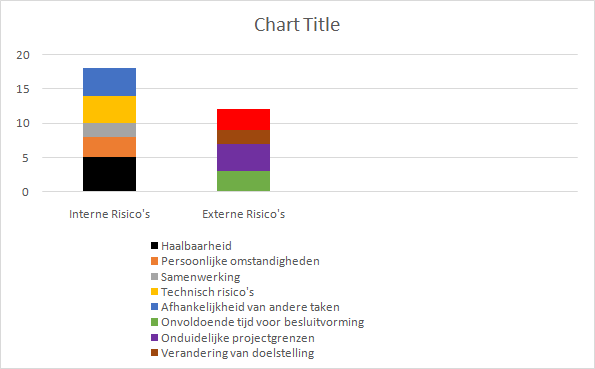
\includegraphics{graph.png}
\\
\\
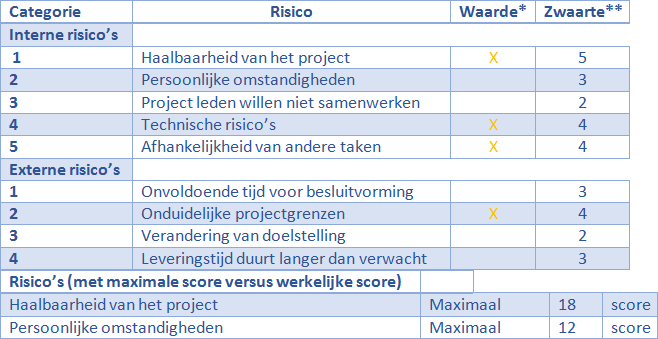
\includegraphics[scale=0.75]{table.png}

\clearpage

\end{document}